% ==================================================
%  Capítulo 3 — Metodología
% ==================================================
\section{Metodología}\label{sec:metodologia}

En esta sección se describe el flujo de trabajo seguido para la generación, procesamiento y consolidación del conjunto de datos utilizado en las etapas posteriores de modelado predictivo y optimización. La metodología se estructura en cinco etapas: descripción del simulador y de las variables del problema, diseño de experimentos, generación de datos mediante simulaciones FDTD, post-procesamiento de las salidas electromagnéticas y consolidación del dataset final. Esta organización separa la generación de la verdad numérica de referencia, proporcionada por FDTD, del uso posterior de modelos subrogados para acelerar la búsqueda de geometrías candidatas.

% --------------------------------------------------
\subsection{Descripción del Simulador}\label{subsec:simulador}

El simulador empleado modela la propagación de un haz de luz láser, implementado como una fuente gaussiana bidimensional, que incide sobre una película de oro (Au) estructurada con nano-rendijas. El código, desarrollado sobre el paquete \texttt{Meep}, ejecuta el siguiente flujo de trabajo para cada configuración geométrica:

\begin{enumerate}
\item \textbf{Construcción de la geometría:} se define el dominio de simulación, se incorporan las regiones dieléctricas correspondientes y se posicionan bloques de oro separados entre sí para formar las nano-rendijas. El tamaño del dominio se calcula dinámicamente en función de la apertura total de cada metalente.

\item \textbf{Inyección de la fuente:} se define una fuente continua de luz con longitud de onda $\lambda = 0.630\;\mu\text{m}$, implementada como un haz gaussiano bidimensional (\texttt{GaussianBeam2DSource}).

\item \textbf{Simulación temporal:} el algoritmo FDTD avanza paso a paso en el tiempo, calculando la propagación, dispersión y transmisión del campo electromagnético al interactuar con la estructura de nano-rendijas. Se utilizan regiones absorbentes (\texttt{mp.Absorber}) en las fronteras para reducir reflexiones numéricas artificiales.

\item \textbf{Captura de datos:} se registra la distribución espacial del campo eléctrico $E_y$ y de la función dieléctrica $\varepsilon$ en el dominio simulado, exportando las salidas crudas en formato HDF5 para su posterior post-procesamiento.

\end{enumerate}

La velocidad de la luz se define computacionalmente como $c = 299{,}792{,}458 \times 10^{-9}\;\mu\text{m/fs}$ para mantener consistencia dimensional con la escala micrométrica empleada por el simulador. El campo monitoreado es $E_y$ en un dominio bidimensional, bajo polarización TM, de acuerdo con la física de excitación plasmónica discutida en la Sección~\ref{subsec:fdtd}.

% --------------------------------------------------
\begin{figure}[H]
    \centering
    \definecolor{primaryBlue}{RGB}{31,90,133}
    \definecolor{secondaryTeal}{RGB}{42,157,143}
    \definecolor{riskRed}{RGB}{182,64,58}
    \definecolor{neutralGray}{RGB}{107,114,128}
    \definecolor{lightPanel}{RGB}{216,222,233}
    \definecolor{goldau}{RGB}{197,138,42}
    \definecolor{goldstroke}{RGB}{99,56,6}
    \colorlet{substrate}{lightPanel}
    \colorlet{substroke}{neutralGray}
    \colorlet{lightgreen}{secondaryTeal}
    \colorlet{annoRed}{riskRed}
    \colorlet{annoBlue}{primaryBlue}
    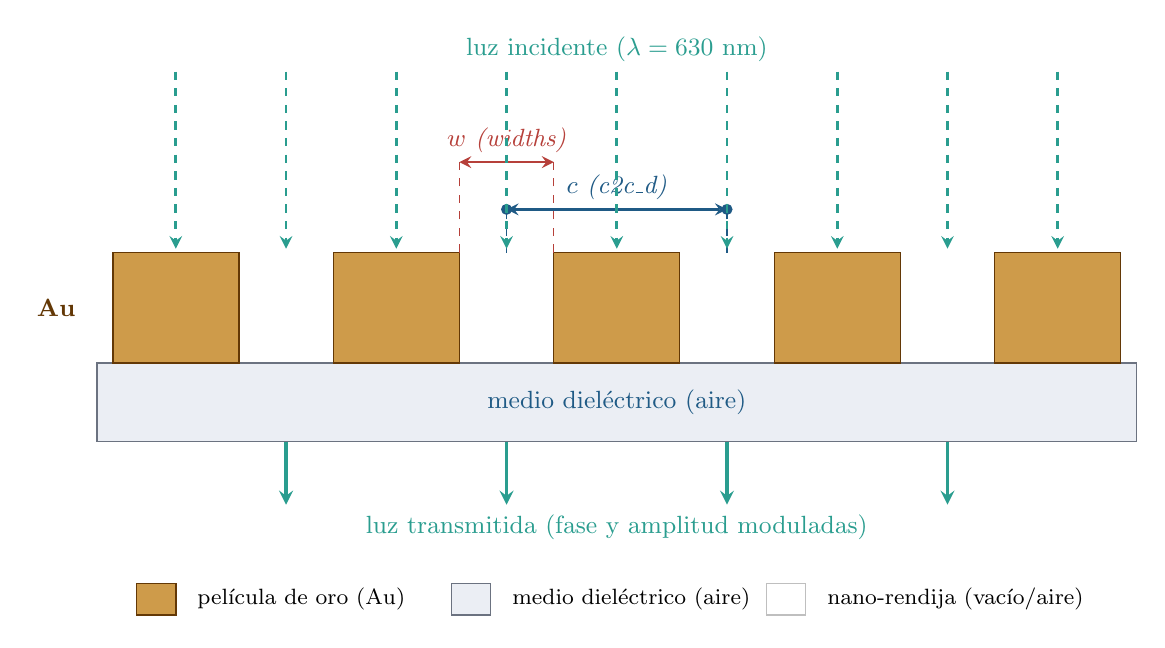
\begin{tikzpicture}[scale=1.0, >=stealth]

  %% Dimensiones base
  \def\ybot{0}
  \def\ysub{1.0}
  \def\yau{\ysub}
  \def\goldh{1.4}
  \def\ytop{\yau+\goldh}   % = 2.4

  %% --- Sustrato dielectrico ---
  \fill[substrate, fill opacity=0.5] (0.0,\ybot) rectangle (13.2,\ysub);
  \draw[substroke, line width=0.6pt] (0.0,\ybot) rectangle (13.2,\ysub);
  \node[font=\small, text=annoBlue] at (6.6, 0.5)
      {medio diel\'ectrico (aire)};

  %% --- 5 bloques de oro identicos (ancho = 1.6 cada uno) ---
  \foreach \xa/\xb in {
      0.2/1.8,
      3.0/4.6,
      5.8/7.4,
      8.6/10.2,
      11.4/13.0}{
    \fill[goldau, fill opacity=0.85] (\xa,\yau) rectangle (\xb,\ytop);
    \draw[goldstroke, line width=0.5pt] (\xa,\yau) rectangle (\xb,\ytop);
  }

  %% Etiqueta Au
  \node[font=\small\bfseries, text=goldstroke, anchor=east]
      at (-0.15, \yau+0.7) {\textbf{Au}};

  %% --- Anotacion widths (rendija 2: 4.6 a 5.8, w=1.2) ---
  \def\xwa{4.6}
  \def\xwb{5.8}
  \def\yannoW{3.55}

  \draw[annoRed, dashed, line width=0.5pt] (\xwa, \ytop) -- (\xwa, \yannoW);
  \draw[annoRed, dashed, line width=0.5pt] (\xwb, \ytop) -- (\xwb, \yannoW);
  \draw[annoRed, <->, line width=0.9pt]
      (\xwa, \yannoW) -- (\xwb, \yannoW);
  \node[font=\small\itshape, text=annoRed, above]
      at ({(\xwa+\xwb)/2}, \yannoW)
      {$w$ \textit{(widths)}};

  %% --- Anotacion c2c_d ---
  \def\xca{5.2}
  \def\xcb{8.0}
  \def\yannoC{2.95}

  \fill[annoBlue] (\xca, \yannoC) circle (2pt);
  \fill[annoBlue] (\xcb, \yannoC) circle (2pt);
  \draw[annoBlue, dashed, line width=0.5pt] (\xca, \ytop) -- (\xca, \yannoC);
  \draw[annoBlue, dashed, line width=0.5pt] (\xcb, \ytop) -- (\xcb, \yannoC);
  \draw[annoBlue, <->, line width=0.9pt]
      (\xca, \yannoC) -- (\xcb, \yannoC);
  \node[font=\small\itshape, text=annoBlue, above]
      at ({(\xca+\xcb)/2}, \yannoC)
      {$c$ \textit{(c2c\_d)}};

  %% --- Luz incidente ---
  \foreach \x in {1.0, 2.4, 3.8, 5.2, 6.6, 8.0, 9.4, 10.8, 12.2}{
    \draw[lightgreen, ->, dashed, line width=1.0pt]
        (\x, 4.7) -- (\x, \ytop+0.05);
  }
  \node[font=\small, text=lightgreen, above] at (6.6, 4.7)
      {luz incidente ($\lambda = 630$ nm)};

  %% --- Luz transmitida ---
  \foreach \x in {2.4, 5.2, 8.0, 10.8}{
    \draw[lightgreen, ->, line width=1.2pt]
        (\x, \ybot) -- (\x, -0.8);
  }
  \node[font=\small, text=lightgreen, below] at (6.6, -0.8)
      {luz transmitida (fase y amplitud moduladas)};

  %% --- Leyenda ---
  \def\yleg{-2.2}
  \fill[goldau, fill opacity=0.85] (0.5,\yleg) rectangle (1.0,\yleg+0.4);
  \draw[goldstroke, line width=0.5pt] (0.5,\yleg) rectangle (1.0,\yleg+0.4);
  \node[font=\footnotesize, anchor=west] at (1.15, \yleg+0.2)
      {pel\'icula de oro (Au)};
  \fill[substrate, fill opacity=0.5] (4.5,\yleg) rectangle (5.0,\yleg+0.4);
  \draw[substroke, line width=0.5pt] (4.5,\yleg) rectangle (5.0,\yleg+0.4);
  \node[font=\footnotesize, anchor=west] at (5.15, \yleg+0.2)
      {medio diel\'ectrico (aire)};
  \fill[white] (8.5,\yleg) rectangle (9.0,\yleg+0.4);
  \draw[black!25, line width=0.5pt] (8.5,\yleg) rectangle (9.0,\yleg+0.4);
  \node[font=\footnotesize, anchor=west] at (9.15, \yleg+0.2)
      {nano-rendija (vac\'io/aire)};

\end{tikzpicture}

    \caption{Esquema de la metalente plasmónica de nano-rendijas. La película de oro
    (Au) está rodeada de aire. La luz incidente
    ($\lambda = 630$~nm) atraviesa las rendijas mediante transmisión óptica extraordinaria
    y emerge con fase y amplitud moduladas. Los parámetros de diseño son el ancho de cada
    rendija $w$ (\texttt{widths}) y la separación centro a centro $c_{2c}$ (\texttt{c2c\_d}).}
    \label{fig:arreglo}
\end{figure}

\subsection{Variables del Problema}\label{subsec:variables}

\subsubsection{Variables de Entrada (Parámetros de Diseño)}

Cada simulación queda definida por los siguientes parámetros geométricos y físicos:

\begin{itemize}
\item \textbf{Anchos de rendija} (\texttt{widths}): vector de $101$ valores, expresados en $\mu$m, que representan el ancho de cada nano-rendija en la película de oro. El rango válido considerado es $20$--$300$~nm. Este intervalo mantiene las rendijas en una escala sub-longitud de onda respecto a $\lambda = 630$~nm y dentro de un rango geométrico compatible con estructuras plasmónicas de nano-rendijas.

\item \textbf{Distancia centro a centro} (\texttt{c2c\_d}): separación entre centros de rendijas adyacentes, expresada en $\mu$m. En este trabajo, dicha separación se mantiene constante para cada metalente, por lo que se representa como un valor escalar por configuración. El rango válido considerado es $150$--$300$~nm, sujeto a las restricciones de no solapamiento y pared mínima de oro entre rendijas.

\item \textbf{Longitud de onda} (\texttt{wavelength}): fija en $0.630\;\mu$m, correspondiente a luz roja en el espectro visible, banda donde el oro exhibe las resonancias plasmónicas superficiales más pronunciadas.

\end{itemize}

Los parámetros de grosor de la película de oro, material, tipo de fuente y configuración general del dominio se mantienen fijos durante el estudio. Por tanto, el espacio de diseño explorado corresponde a una familia parametrizada de metalentes de $101$ nano-rendijas, no al conjunto completo de geometrías posibles.

\subsubsection{Variables de Salida (Respuesta Óptica)}

Las salidas crudas del simulador son tensores multidimensionales del campo eléctrico $E_y$ y de la función dieléctrica $\varepsilon$, almacenados en formato HDF5. A partir de estas salidas se realiza un post-procesamiento para extraer descriptores ópticos y construir las variables utilizadas en las etapas de modelado:

\begin{itemize}
\item \textbf{Campo óptico focal complejo:} se identifica dinámicamente el plano focal o plano de máxima intensidad y se extraen perfiles transversales asociados al campo transmitido. En el enfoque final de modelado, la respuesta objetivo del surrogate se representa mediante perfiles de amplitud y fase del campo focal, re-muestreados a una longitud fija.

\item \textbf{Calidad de enfoque} ($R^2$): se ajusta un polinomio de segundo grado a la trayectoria de máxima intensidad ($|E_y|^2$) a lo largo del eje de propagación. El coeficiente de determinación $R^2$ se utiliza como métrica operativa para cuantificar la regularidad parabólica asociada al enfoque. En este trabajo, el umbral $R^2 \geq 0.90$ define el criterio práctico de éxito para seleccionar candidatos, siempre sujeto a confirmación mediante FDTD.

\item \textbf{Transmitancia} ($T$): descriptor óptico asociado a la fracción de energía transmitida a través de la estructura, evaluado a partir del campo simulado. En este trabajo se conserva como métrica física relevante, aunque el modelo subrogado final se centra principalmente en la predicción del campo focal complejo y en métricas derivadas de calidad de enfoque.

\item \textbf{Perfil de fase desenvuelta} ($\phi$): perfil transversal de fase extraído del campo eléctrico complejo en el plano focal identificado dinámicamente. La fase se desenvuelve y se procesa para obtener una representación comparable entre simulaciones.

\end{itemize}

Así, $R^2$ y $T$ se interpretan como descriptores derivados y criterios de evaluación, mientras que la amplitud y fase focales constituyen la representación densa que alimenta el modelo subrogado final.

% --------------------------------------------------
\subsection{Diseño de Experimentos}\label{subsec:doe}

\subsubsection{Perfiles de Anchos}

El perfil de anchos define cómo varía el ancho de cada rendija a lo largo de la metalente, modificando localmente la fase y la amplitud del campo transmitido. Para generar un conjunto inicial de geometrías físicamente plausibles y con diversidad estructural, se emplearon seis familias parametrizadas de perfiles:

\begin{itemize}
\item \textbf{Parabólico:} $w(x) = w_{\min} + (w_{\max} - w_{\min}) \cdot a \cdot x^2$. Permite explorar configuraciones inspiradas en perfiles de fase de lentes convergentes, donde la variación geométrica crece con la distancia al centro.

\item \textbf{Gaussiano:} $w(x) = w_{\min} + (w_{\max} - w_{\min}) \cdot \exp\!\left(-x^2 / 2\sigma^2\right)$. Introduce perfiles suaves tipo campana, útiles para evaluar respuestas con mayor peso geométrico cerca de la región central.

\item \textbf{Lineal:} $w(x) = w_{\min} + (w_{\max} - w_{\min}) \cdot |x \cdot s|$. Permite explorar variaciones monotónicas respecto al centro, asociadas a respuestas de red o desviación preferencial del campo.

\item \textbf{Constante:} $w(x) = k$. Representa arreglos de rendijas idénticas y funciona como una línea base geométrica para contrastar contra perfiles espacialmente variables.

\item \textbf{Sinusoidal:} $w(x) = w_{\min} + (w_{\max} - w_{\min}) \cdot \tfrac{1}{2}(1 + \cos(2\pi f x + \varphi))$. Introduce modulaciones periódicas capaces de generar patrones de interferencia y difracción más complejos.

\item \textbf{Escalonado:} zonas de ancho constante por segmentos ($2$--$5$ zonas), con suavizado por promedio móvil. Esta familia permite representar perfiles segmentados, cercanos a diseños discretizados y potencialmente más simples de fabricar.

\end{itemize}

La diversidad de perfiles busca que el conjunto de datos contenga ejemplos con diferentes tipos de respuesta óptica, incluyendo configuraciones que enfocan y configuraciones que no enfocan. No obstante, este diseño de experimentos no cubre el espacio completo de posibles geometrías de $101$ rendijas independientes; más bien explora un subconjunto estructurado y parametrizado del espacio de diseño. Esta decisión hace viable la generación de datos, pero también limita la capacidad del modelo para generalizar hacia geometrías arbitrarias fuera del dominio muestreado.

\subsubsection{Restricciones Físicas}

Toda configuración generada, independientemente del perfil o semilla aleatoria, satisface las siguientes restricciones geométricas:

\begin{enumerate}
    \item $0.020 \leq w_i \leq 0.300\;\mu$m \quad (anchos de rendija en régimen sub-longitud de onda).
    \item $0.150 \leq c_{2c} \leq 0.300\;\mu$m \quad (separación centro a centro entre rendijas adyacentes).
    \item $c_{2c} - \tfrac{1}{2}(w_j + w_{j+1}) \geq 0.020\;\mu$m \quad (pared mínima de oro entre rendijas).
    \item $0.1 \leq w_i/c_{2c} \leq 0.5$ \quad (factor de llenado en el régimen de resonancia óptima para EOT).
\end{enumerate}

Estas restricciones evitan configuraciones físicamente inválidas, como solapamiento entre rendijas o paredes metálicas demasiado delgadas, y acotan el espacio de búsqueda a geometrías compatibles con el simulador y con las hipótesis del estudio.

\subsubsection{Muestreo del Espacio de Diseño}

Aunque una metalente con $101$ rendijas podría describirse, en principio, mediante $101$ anchos y $100$ separaciones independientes, en este diseño de experimentos la separación centro a centro se mantiene constante por metalente. Por ello, cada geometría se representa mediante un vector de $102$ componentes: $101$ anchos de rendija más un valor escalar de separación $c_{2c}$.

La dimensionalidad efectiva del conjunto generado es menor que $102$, ya que los anchos no se muestrean de manera completamente independiente. Cada configuración queda determinada por una familia de perfil, el valor de $c_{2c}$ y un número reducido de parámetros internos que definen la forma del perfil, como la amplitud $a$ del parabólico, el ancho $\sigma$ del gaussiano, la pendiente $s$ del lineal, o la frecuencia $f$ y la fase $\varphi$ del sinusoidal. Las configuraciones se generan mediante un script de muestreo que busca cubrir de manera amplia el dominio permitido de estos parámetros bajo las restricciones físicas establecidas.

% --------------------------------------------------
\subsection{Generación de Datos}\label{subsec:generacion}

\subsubsection{Estrategia de Generación y Post-procesamiento}

Los archivos HDF5 crudos generados por Meep pesan aproximadamente $1$~GB cada uno. Para manejar las restricciones de almacenamiento, se implementó una estrategia denominada \textit{Compute, Extract and Destroy}: dentro del mismo trabajo de ejecución, el simulador genera el tensor electromagnético, un módulo de post-procesamiento extrae los descriptores ópticos de interés y finalmente el archivo HDF5 original se elimina.

En las primeras etapas, los descriptores extraídos incluían métricas escalares como $R^2$, transmitancia $T$ y fase desenvuelta $\phi$. Tras el re-encuadre metodológico del proyecto, el post-procesamiento se amplió para conservar una representación más densa de la respuesta óptica: perfiles de amplitud y fase del campo focal, re-muestreados a longitud fija. Estos descriptores se almacenan en archivos JSON ligeros, lo que permite conservar la información necesaria para el modelado sin mantener los archivos HDF5 completos.

El módulo de extracción de \textit{features} opera sobre el tensor de campo $E_y$ en cuatro pasos principales: (i) rastrea los picos de intensidad máxima ($|E_y|^2$) a lo largo del eje de propagación; (ii) ajusta una parábola a esa trayectoria para obtener el coeficiente $R^2$; (iii) identifica dinámicamente el plano focal o plano de máxima intensidad; y (iv) extrae en dicho plano los perfiles transversales de amplitud, fase desenvuelta y descriptores derivados como la transmitancia $T$. Estas variables corresponden a las salidas descritas en la Sección~\ref{subsec:variables}.


\subsubsection{Lotes de Simulación}

La generación de datos para el entrenamiento se ejecutó en dos lotes principales, ambos en el régimen de $101$ rendijas:

\begin{itemize}
\item \textbf{Lote 1 (Clúster Lab-SB, CIMAT):} $500$ simulaciones (\texttt{sim\_001} a \texttt{sim\_500}) con semilla $\texttt{seed}=42$, ejecutadas mediante \textit{Job Arrays} de SLURM con paralelismo controlado. Se emplearon cuatro tipos de perfil de anchos: parabólico, gaussiano, lineal y constante.

\item \textbf{Lote 2 (Servidor privado):} $500$ simulaciones adicionales (\texttt{sim\_501} a \texttt{sim\_1000}) con semilla $\texttt{seed}=2026$, ampliando las familias de perfiles para incluir perfiles sinusoidales y escalonados, además de los cuatro perfiles originales. Se ejecutaron secuencialmente mediante un script orquestador, con los mismos módulos de simulación y extracción de \textit{features}.

\end{itemize}

El uso de semillas distintas y familias de perfiles adicionales buscó ampliar la cobertura del espacio parametrizado de diseño. No obstante, esta estrategia no garantiza cobertura global del espacio completo de geometrías posibles, sino una exploración más diversa dentro del dominio definido por el diseño de experimentos. Adicionalmente, la investigadora responsable proporcionó un conjunto de $200$ simulaciones (\texttt{Simulation\_XXX}) en un régimen físico distinto, con número de rendijas y separaciones fuera del rango considerado en este estudio. Por esta razón, dichas simulaciones no se incluyen en el entrenamiento del modelo final y se conservan únicamente como referencia cualitativa externa.

% --------------------------------------------------
\subsection{Infraestructura Computacional}\label{subsec:infraestructura}

Las simulaciones se ejecutaron en dos plataformas de cómputo. El clúster Lab-SB del Laboratorio de Supercómputo del Bajío (CIMAT) proporcionó nodos de cómputo y gestión de trabajos mediante SLURM, permitiendo la ejecución paralela del primer lote. El segundo lote se ejecutó en un servidor privado con GPU dedicada, operando de forma secuencial con tolerancia automática a fallos y reanudación tras interrupciones. En ambos casos se utilizó el mismo entorno base de software, incluyendo Meep, NumPy, SciPy y H5py, con el objetivo de mantener consistencia en la generación y post-procesamiento de los resultados.

% --------------------------------------------------
\subsection{Consolidación del Dataset}\label{subsec:consolidacion}

\subsubsection{Re-encuadre del Objetivo}\label{subsubsec:reencuadre}

Una auditoría temprana del enfoque, desarrollada en el análisis exploratorio (Sección~\ref{sec:eda}), motivó un cambio en la representación del objetivo de aprendizaje que se detalla en la Sección~\ref{sec:modelado}. En lugar de reducir cada simulación a un escalar de calidad ($R^2$) o a una etiqueta binaria, se conservó una representación densa de la respuesta óptica: el campo complejo en el plano focal, descrito mediante amplitud $|E|(y)$ y fase $\Phi(y)$, re-muestreadas a una longitud fija de $1{,}024$ puntos.

Con ello, el dataset conserva la información de todas las simulaciones, incluidas aquellas que no producen enfoque satisfactorio, y no solo la escasa región de alto $R^2$. Esta representación densa no elimina las limitaciones asociadas al tamaño del conjunto, pero aprovecha información que el objetivo escalar dejaba sin uso.

\subsubsection{Estructuración del Dataset}

De cada registro consolidado se integra el identificador de la simulación, el vector geométrico $\mathbf{x} \in \mathbb{R}^{102}$, compuesto por $101$ anchos y una separación centro a centro $c_{2c}$ constante por metalente, la amplitud y fase del campo focal re-muestreadas a $1{,}024$ puntos, y el coeficiente $R^2$ asociado al perfil de intensidad. En las simulaciones base, la geometría proviene de los archivos de diseño de experimentos y la respuesta óptica de los JSONs procesados; en las confirmaciones FDTD, ambos elementos se conservan en los registros confirmados.

La longitud de $1{,}024$ puntos se eligió por ser la potencia de dos inmediatamente superior al máximo observado de $N_y = 1{,}023$ puntos transversales en el plano focal del dataset. El valor de $N_y$ varía entre simulaciones porque el dominio FDTD se dimensiona dinámicamente en función de la apertura de cada metalente. Esta elección permite representar todos los perfiles con una longitud común sin pérdida de resolución por submuestreo respecto al máximo observado.

El coeficiente $R^2$ se conserva como métrica de referencia, criterio operativo de selección y variable de estratificación para las particiones, pero no como objetivo binario del modelo final. El objetivo principal del surrogate final corresponde a la predicción de los perfiles de amplitud y fase focales.

\subsubsection{Estratificación y Partición}

El dataset oficial consolida $1{,}110$ simulaciones: $1{,}000$ provienen del diseño de experimentos inicial (\texttt{sim\_XXX}), $90$ del ciclo de mejora inicial (el subconjunto con geometría recuperable de las ${\sim}180$ simulaciones del ciclo activo descrito en la Sección~\ref{subsec:enfoque_v1}) y $20$ de las dos primeras iteraciones de diseño inverso confirmadas por FDTD. Las confirmaciones posteriores (iteración~5 y el refinamiento por hill-climbing, Sección~\ref{sec:resultados}) son cronológicamente posteriores al congelado del dataset, por lo que se reportan como resultados sin reincorporarse al entrenamiento. Para preservar representación de la escasa región de alto $R^2$ en cada partición, se aplicó estratificación por bandas de $R^2$ ($<0.30$, $[0.30,0.70)$, $[0.70,0.85)$, $\geq 0.85$) con semilla fija ($\texttt{seed}=42$) y proporciones $70\%/15\%/15\%$.

Las geometrías confirmadas durante las iteraciones de diseño inverso se incorporan al conjunto de entrenamiento para mantener las particiones de validación y prueba como conjuntos de evaluación independientes respecto al proceso final de selección de candidatos. Esta decisión evita evaluar el modelo sobre geometrías que ya fueron utilizadas dentro del ciclo de diseño asistido. La distribución resultante es $781$ / $161$ / $168$ para entrenamiento, validación y prueba.

\begin{table}[H]
\centering
\small
\begin{tabular}{lcccc}
\toprule
\textbf{Banda $R^2$} & \textbf{$<0.30$} & \textbf{$[0.30,0.70)$} & \textbf{$[0.70,0.85)$} & \textbf{$\geq 0.85$} \\
\midrule
Entrenamiento & 527 & 200 & 35 & 19 \\
Validación & 112 & 42 & 6 & 1 \\
Prueba & 114 & 43 & 8 & 3 \\
\bottomrule
\end{tabular}
\caption{Distribución del dataset ($1{,}110$ simulaciones) por partición y banda de $R^2$.}
\label{tab:particion}
\end{table}
